\section{(Un)abhängigkeit} \label{sec:unabhangigkeit}
In vielen Fällen besagt die Intuition über verschiedene Zufallsexperimente / Ereignisse, dass diese sich \emph{nicht} gegenseitig beeinflussen. Für solche $A,B \in \F$ mit $\P(A) > 0, \P(B) > 0$ sollte gelten
\begin{align*}
\P(A\mid B) = \P(A), \quad \P(B\mid A) = \P(B).
\end{align*}

\begin{definition}[(Stochastische) Unabhängigkeit]
	\proplbl{3_11}
	Sei $(\O, \F, \P)$ Wahrscheinlichkeitsraum. Zwei Ereignisse $A,B \in \F$ heißt \begriff{(stochastisch) unabhängig bezüglich $\P$}, falls
	\begin{align*}
		\P(A\cap B) = \P(A)\P(B).
	\end{align*}
	Wir schreiben auch $A \upmodels B$.
\end{definition}
\begin{example}
	\proplbl{3_12}
	Würfeln mit 2 fairen, sechsseitigen Würfeln:
	\begin{align*}
	\O &= \set{(i,j) \mid i,j \in\set{1,\dots,n}},\quad \F = \pows(\O), \quad \P = \Gleich(\O)
	\intertext{Betrachte}
	A:= \set{(i,j) \in \O, i \text{ gerade}}\\
	B:= \set{(i,j) \in \O, j \le 2}.
	\end{align*}
	In diesem Fall, erwarten wir intuitiv Unabhängigkeit von $A$ und $B$.\\
	In der Tat ist % start using \P instead of \Propb!
	\begin{align*}
	\P(A) = \frac{1}{2}, \quad \P(B) = \frac{1}{3} \und \P(A\cap B) = \frac{1}{6}
	\intertext{was}
	\P(A \cap B) = \P(A) \P(B)
	\end{align*}
	erfüllt. Betrachte nun
	\begin{align*}
	C&:= \set{(i,j) \in \O \mid i + j = 7}\\
	D&:= \set{(i,j) \in \O \mid i = 6}
	\intertext{dann gilt}
	\P(C) = \frac{1}{6}, \quad \P(D) = \frac{1}{6}
	\intertext{und wegen $C \cap D = \set{(6,1)}$ folgt}
	\P(C\cap D) = \frac{1}{36} = \frac{1}{6} \frac{1}{6} = \P(C) \cdot \P(D)
	\end{align*}
	$C$ und $D$ sind also \emph{stochastisch} unabhängig, obwohl eine kausale Abhängigkeit vorliegt!
\end{example}

\begin{definition}[Unabhängigkeit bezüglich $\P$]
	\proplbl{3_13}
	Sei $(\O, \F, \P)$ Wahrscheinlichkeitsraum und $I \neq \emptyset$ endliche Indexmenge. Dann heißt die Familie $(A_i)_{i \in I}$ von Ereignissen in $\F$ \begriff{unabhängig bezüglich $\P$}, falls für alle $J \subseteq I, J \neq \emptyset$ gilt:
	\begin{align*}
		\P\brackets{\bigcap_{i\in J}A_i} = \prod_{i\in J} \P(A_i)
	\end{align*}
	Offensichtlich impliziert die Unabhängigkeit einer Familie die paarweise Unabhängigkeit je zweier Familienmitglieder nach \propref{3_11}. Umgekehrt gilt dies nicht!
\end{definition}

\begin{example}[Abhängigkeit trotz paarweiser Unabhängigkeit]
	\proplbl{3_14}
	Betrachte zweifaches Bernoulliexperiment mit Erfolgswahrscheinlichkeit $\sfrac{1}{2}$, d.h.
	\begin{align*}
		\O = \set{0,1}^2, \quad \F = \pows(\O), \quad \P = \Gleich(\O)
		\intertext{sowie}
		A &= \set{1}\times \set{0,1} \qquad \text{(Münzwurf: erster Wurf ist Zahl)}\\
		B &= \set{0,1}\times \set{1} \qquad \text{(Münzwurf: zweiter Wurf ist Zahl)}\\
		C &= \set{(0,0), (1,1)} \qquad \text{(beide Würfe haben selbes Ergebnis)}
	\end{align*}
	Dann gelten $\P(A) = \frac{1}{2} = \P(B) = \P(C)$ und
	\begin{align*}
		\P(A\cap B) = \P(\set{(1,1)}) = \frac{1}{4} = \P(A)\P(B)\\
		\P(A\cap C) = \P(\set{(1,1)}) = \frac{1}{4} = \P(A)\P(C)\\
		\P(B\cap C) = \P(\set{(1,1)}) = \frac{1}{4} = \P(B)\P(C)
	\end{align*}
	also paarweise Unabhängigkeit. Aber
	\begin{align*}
	\P(A\cap B \cap C) = \P(\set{(1,1)}) = \frac{1}{4} \neq \P(A)\P(B)\P(C)
	\end{align*}
	und $A,B,C$ sind \emph{nicht} stochastisch unabhängig.
\end{example}

\begin{definition}[Unabhängige $\sigma$-Algebren]
	\proplbl{3_15}
	% started using \O for \Omega and \Gen for this special generating set E_i
	Seien $(\O, \F,\P)$ Wahrscheinlichkeitsraum, $I \neq \emptyset$ Indexmenge und $(E_i, \Gen_i)$ Messräume
	\begin{enumerate}
		\item Die Familie $\F_i \subset \F, i \in I$, heißen \begriff{unabhängig}, wenn für die $J \subseteq I, J \neq \emptyset, \abs{J} < \infty$ gilt
		\begin{align*}
			\P\brackets{\bigcap_{i \in J} A_i} = \prod_{i\in J} \P(A_i) \qquad \text{ für beliebige } A_i \in \F_i, i \in J
		\end{align*}
		\item Die Zufallsvariable $X_i: (\O, \F) \to (E_i, \Gen_i), i \in I$, heißen \begriff{unabhängig}, wenn die $\sigma$-Algebren
		\begin{align*}
		\sigma(X_i) = X^{-1}(\Gen_i) = \set{\set{X_i \in F} \colon F \in \Gen_i}, \quad i \in I
		\end{align*}
		unabhängig sind.
	\end{enumerate}
\end{definition}

\begin{lemma}[Zusammenhang der Definitionen]
	\proplbl{3_16}
	Sei $(\O,\F,\P)$ Wahrscheinlichkeitsraum, $I \neq \emptyset, A \in \F, i \in I$. 
	Die folgenden Aussagen sind äquivalent:
	\begin{enumerate}
		\item Die Ereignisse $A_i, i \in I$ sind unabhängig. 
		\item Die $\sigma$-Algebren $\sigma(A_i), i \in I$ sind unabhängig.
		\item Die Zufallsvariablen $\indi_{A_i}, i \in I$ sind unabhängig.
	\end{enumerate}
\end{lemma}
\begin{proof} %TODO add ref?
	Da die Unabhängigkeit über endliche Teilemengen definiert ist, können wir oBdA $I = \set{1, \dots, n}$ annehmen. 
	\begin{itemize}
		\item Da $\sigma(\indi_{A_i}) = \sigma(A_i)$ folgt die Äquivalenz von 2. und 3. direkt aus \propref{3_15}.
		\item Zudem ist 2. $\to$ 1. klar!
		\item Für 1 $\to$ 2. genügt es zu zeigen, dass
		\begin{align*}
			A_1, \dots, A_n \text{ unabhängig } &\Rightarrow B_1, \dots, B_n \text{ unabhängig mit } B_i \in \set{\emptyset, A_i, A_i^C, \O}.
			\intertext{Rekursiv folgt dies bereits aus}
			A_1,\dots, A_n \text{ unabhängig } &\Rightarrow B_1, A_2, \dots, A_n \text{ unabhängig mit } B_1 \in \set{\emptyset, A_1, A_1^C, \O}.
		\end{align*}
		Für $B_1 \in \set{\emptyset, A_1, \O}$ ist dies klar.\\
		Sei also $B_1 = A_1^C$ und $J \subseteq I, J \neq \emptyset$. Falls $1 \not \in J$, ist nichts zu zeigen. Sei $1 \in J$, dann gilt mit
		\begin{align*}
			A &= \bigcap_{i\in J, i \neq 1} A_i
			\intertext{sicherlich}
			\P\brackets{A_1^C \cap A} &= \P(A \setminus (A_1 \cap A))\\
			&= \P(A) - \P(A_1 \cap A)\\
			&= \prod_{i\in J\setminus \set{1}} \P(A_i) - \prod_{i\in J}(A_i)\\
			&= (1- \P(A_1))\prod_{i\in J\setminus \set{1}} \P(A_i)\\
			&= \P\brackets{A_1^C})\prod_{i\in J\setminus \set{1}} \P(A_i)
		\end{align*} 
	\end{itemize}
\end{proof}
Insbesondere zeigt \propref{3_16}, dass wir in einer Familie unabhängiger Ereignisse beliebig viele Ereignisse durch ihr Komplement, $\emptyset$ oder $\O$ ersetzen können, ohne die Unabhängigkeit zu verlieren.
\begin{proposition}
	\proplbl{3_17}
	Sei $(\O, \F, \P)$ Wahrscheinlichkeitsraum und $\F_i \subseteq \F, i \in I$, seien $\cap$-stabile Familien von Ereignissen. Dann gilt
	\begin{align*}
	\F_i, i \in I \text{ unabhängig } \iff \sigma(\F_i), i \in I \text{ unabhängig}. 
	\end{align*}
\end{proposition}
\begin{proof}
	oBdA sei $I = \set{1, \dots, n}$ und $\O \in \F_i, i \in I$.
	\begin{itemize}
		\item $\Leftarrow$: trivial, da $\F_i \subseteq \sigma(\F_i)$ und das Weglassen von Mengen erlaubt ist.
		\item $\Rightarrow$: zeigen wir rekursiv
		\begin{enumerate}
			\item Wähle $F_i \in \F_i, i = 2, \dots,n$ und defniere für $F \in \sigma(\F_i)$ die endlichen Maße
			\begin{align*}
				\mu(F) = \P\brackets{ F \cap F_2 \cap \cdots \cap F_n} \und \nu(F) = \P(F) \, \P(F_2) \, \dots \, \P(F_n)
			\end{align*}
			\item Da die Familien $\F_i$ unabhängig sind, gilt
			$\mu\mid_{\F_1} = \nu\mid_{\F_1}$.
			Nach dem Eindeutigkeitssatz für Maße (\propref{1_1_9}) folgt $\mu\mid_{\sigma(\F_1)} = \nu\mid_{\sigma(\F_1)}$ also
			\begin{align*}
				\P\brackets{ F \cap F_2 \cap \cdots \cap F_n} = \P(F) \P(F_2) \dots \P(F_n)
			\end{align*}
			für alle $F \in \sigma(\F_i)$ und $F_i \in \F_i, i = 1, \dots, n$. Da $\O \in \F_i$ für alle $i$ gilt die erhaltene Produktformel für alle Teilemengen $J \subseteq I$.\\
			Also sind
			\begin{align*}
			\sigma(\F_1), \F_2, \dots, \F_n \text{ unabhängig}
			\end{align*}
			\item Wiederholtes Anwenden von $1$ und $2$ liefert den Satz.
		\end{enumerate}
	\end{itemize}
\end{proof}
Mit \propref{3_17} folgen:
\begin{conclusion}
	\proplbl{3_18}
	Sei $(\O,\F,\P)$ Wahrscheinlichkeitsraum und
	\begin{align*}
		\F_{i,j} \subseteq \F, \quad 1 \le i \le n, 1 \le j \le m(i)
	\end{align*}
	unabhängige, $\cap$-stabile Familien.
	Dann sind auch
	\begin{align*}
		\G_i = \sigma(\F_{i,1}, \dots , \F_{i,m(i)}), \quad 1 \le i \le n
	\end{align*}
	unabhängig.
\end{conclusion}
\begin{conclusion}
	\proplbl{3_19}
	Sei $(\O,\F,\P)$ Wahrscheinlichkeitsraum und
	\begin{align*}
		X_{ij}: \O \to E, \quad 1 \le i \le n, 1 \le j \le m(i)
	\end{align*}
	unabhängige Zufallsvariablen. Zudem seien $f_i: E^{m(i)} \to \R$ messbar. Dann sind auch die Zufallsvariablen
	\begin{align*}
		f_i(X_{i,1}, \dots, X_{i,m(i)}), \quad 1 \le i \le n
	\end{align*}
	unabhängig.
\end{conclusion}
\begin{example}
	\proplbl{3_20}
	$X_1, \dots, X_n$ unabhängige reelle Zufallsvariablen. Dann sind auch
	\begin{align*}
	Y_1 = X_1, Y_2 = X_2 + \cdots + X_n
	\end{align*}
	unabhängig.
\end{example}
% % % % % % % % % % % % % % % % % 7th lecture % % % % % % % % % % % % % % % % % % %
\begin{proof}[\propref{3_18}]
	OBdA sei $\Omega \in \F_{i,j} \forall i,j$. Dann sind die Familien:
	\begin{align*}
		\F_i^{\cap} := \set{F_{i,1} \cap \dots \cap F_{i,m(i)} \mid F_{i,j} \in \F_{i,j}, 1 \le j \le m(i)}, 1 \le i \le n
	\end{align*}
	$\cap$-stabil, unabhängig und es gilt: $\F_{i,1}, \dots, \F_{i,m(i)} \subseteq \F_i^{\cap}$ ($\nearrow$ HA)! Nach \propref{3_17} sind auch $\sigma(\F_i^{\cap})$ unabhängig. Damit folgt die Behauptung, da $\sigma(\F_i^{\cap}) = \G_i$:
	\begin{align*}
		\F_{i,1}, \dots, \F_{i,m(i)} \subseteq \F_i^{\cap} \subseteq \sigma(\F_{i,1}, \dots, \F_{i,m(i)}) = \G_i\\
		\Rightarrow \G = \sigma(\F_{i,1}, \dots, \F_{i,m(i)}) \subseteq \sigma(\F_i^{\cap}) \subseteq \G_i.
	\end{align*}
\end{proof}
\begin{proof}[\propref{3_19}]
	Setze $\F_{i,j} = \sigma(X_{i,j})$ und $\G_i = \sigma(\F_{i,1}, \dots, \F_{i,m(i)})$, dann sind nach \propref{3_18} die $\G_i, i = 1,\dots,n$ unabhängig. Zudem ist
	\begin{align*}
	Y_i := f_i(X_{i,1}, \dots, X_{i,m(i)})
	\end{align*}
	$\G_i$ messbar, also $\sigma(Y_i) \subseteq \G_i$. Damit erben die $Y_i$ die Unabhängigkeit der $\G_i$.
\end{proof}
\begin{proposition}[Unabhängigkeit von Zufallsvariablen]
	\proplbl{3_21}
	$(\O, \F, \P)$ Wahrscheinlichkeitsraum und $X_1, \dots, X_n: (\O,\F) \to (E, \Gen)$ Zufallsvariablen. Dann sind die folgenden Aussagen äquivalent:
	\begin{enumerate}
		\item $X_1, \dots, X_n$ sind unabhängig \label{prop:unabhZV1}
		\item $\P(X_1 \in A_1, \dots, X_n \in A_n) = \prod_{i=1}^n \P(X_i \in A_i)\quad \forall A_1, \dots, A_n \in \Gen$. \label{prop:unabhZV2}
		\item Die gemeinsame Verteilung der $X_i$ entspricht dem Produktmaß der einzelnen Verteilungen \label{prop:unabhZV3}
		\begin{align*}
			\P_{X_1, \dots, X_n} = \bigotimes_{i=1}^n \P_{X_i}
		\end{align*}
	\end{enumerate}
\end{proposition}
\begin{proof}
	Per Ringschluss:
	\begin{enumerate} %TODO add labels
		\item[1 $\Rightarrow$ 2:] Seien $A_1, \dots, A_n\in E$ beliebig, dann gilt per Definition
		\begin{align*} % für Rechtecke
			\P_{X_1, \dots, X_n}(A_1 \times \dots \times A_n) &= \P(X_1 \in A_1, \dots, X_n \in A_n)\\
			&= \P\brackets{\bigcap_{i=1}^n \set{X_i \in A_i}}\\
			\overset{\text{unabh}}&{=} \prod_{i=1}^n \P(X_i \in A_i)\\
			&= \prod_{i=1}^n \P_{X_i}(A_i) = \brackets{\bigotimes_{i=1}^n \P_{X_i}} (A_1 \times \dots \times A_n) 
		\end{align*} 
		\item[2 $\Rightarrow$ 3:] Aus der obigen Rechnung sehen wir, dass 2 bereits 3 impliziert für alle Rechtecke: $\bigtimes_{i = 1}^n A_i$. Da die Familie der Rechtecke $\cap$-stabil ist und $\E^{\otimes n}$ erzeugt, folgt die Aussage aus dem Eindeutigkeitssatz für Maße \propref{1_9}.
		\item[3 $\Rightarrow$ 1:] Sei $J \subseteq \set{1,\dots,n}$ und setze
		\begin{align*}
			A_i &:= \begin{cases}
			\text{ beliebig }  &\text{ in }\E, i \in J\\
			E & i \notin J.
			\end{cases}
			\intertext{Dann}
			\P(X_i \in A_i, i \in J) &= \P(X_i \in A_i, i = 1, \dots,n)\\
			&= \prod_{i=1}^n \P(X_i \in A_i)\\
			&= \prod_{i\in J} \P(A_i \in A_i).
		\end{align*}
	\end{enumerate}
\end{proof}
\begin{example}
	\proplbl{3_22}
	Im Urnenmodell mit Zurücklegen hat der Vektor $X = (X_1, \dots, X_n)$ mit $X_i = $ Farbe im $i$-ten Zug als Zähldichte die Produktdichte der $X_i$. Die $X_1, \dots, X_n$ sind also unabhängig.
\end{example}
\subsection{Konstruktion unabhängiger Zufallsvariablen}
Kapitel \ref{chapter1}: Zu beliebiger Wahrscheinlichkeitsverteilung $\P_X$ existiert Wahrscheinlichkeitsraum mit Zufallsvariable $X$ auf diesem Wahrscheinlichkeitsraum, so dass $X \sim \P_X$.
\begin{enumerate}
	\item Seien $\P_{X_1}, \dots, \P_{X_n}$ Wahrscheinlichkeitsverteilungen auf $(E, \E)$. Gibt es einen Wahrscheinlichkeitsraum $(\O, \F, \P)$ und Zufallsvariablen $X_1, X_2$ unabhängig, so dass $X_1 \sim \P_{X_1}$? \label{konstruktionunabh:ZV:qu_1}
	\item Wie kann ich beliebig (unendlich) viele unabhängige Zufallsvariablen konstruieren? \label{konstruktionunabh:ZV:qu_2}
\end{enumerate}
Wir beginnen mit \ref{konstruktionunabh:ZV:qu_1}:\\
Konstruiere zwei Wahrscheinlichkeitsräume $(\O_i, \F_i, \P_i), i = 1,2$ und Zufallsvariablen $X_1, X_2 \mit X_i \sim \P_{X_i}$. Auf dem Produktraum
\begin{align*}
	\O = \O_1 \times \O_2, \quad \F := \F_1 \otimes \F_2 \und \P = \P_1 \otimes \P_2
	\intertext{ definiere}
	X'_1: \O_1 \times \O_2 \to E\colon (\omega_1, \omega_2) \mapsto X_1(\omega_1)\\
	X'_2: \O_1 \times \O_2 \to E\colon (\omega_1, \omega_2) \mapsto X_2(\omega_2)
\end{align*}
Dann gilt für beliebige Ereignisse: $F_1, F_2 \in \E$
\begin{align*}
	\underbrace{\set{X'_1 \in F_1} \cap \set{X'_2 \in F_2}}_{\supseteq \O = \O_1 \times \O_2} = \underbrace{\set{X_1 \in F_1}}_{\supseteq \O_1} \times \underbrace{\set{X_2 \in F_2}}_{\supseteq \O_2} \in \F_1 \times \F_2
\end{align*}
und damit folgt die Messbarkeit der Abbildungen $X'_1, X'_2$, d.h. $X'_1, X'_2$ sind Zufallsvariablen auf $(\O, \F)$. Zudem gilt
\begin{align*}
	\P(X'_1 \in F_1, X'_2 \in F_2) &= \P_1 \otimes \P_2 \brackets{\set{X_1 \in F_1} \times \set{X_2 \in F_2}}\\
	&= \P_1 (X_1 \in F_1) \P_2(X_2 \in F_2),
	\intertext{also}
	\P(X'_i \in F_i) &= \P_i (X'_i \in F_i)
\end{align*}
sowie nach \propref{3_23:prop:Kolmo} $X'_1 \upmodels X'_2$.\\
Wenn $(\O_2, \F_1, \P_1) = (\O_2, \F_2, \P_2)$, so liefert die obige Konstruktion zwei unabhängige Zufallsvariablen auf einem Wahrscheinlichkeitsraum. Andernfalls können wir auf den Produktraum ausweichen und $X'_i$ anstelle von $X_i$ betrachten. Die obige Konstruktion lässt sich direkt auf \emph{endlich} viele Zufallsvariablen übertragen.\\
Zu \ref{konstruktionunabh:ZV:qu_2}: 
\begin{proposition}[Satz von \person{Kolmogorov}]
	\proplbl{3_23:prop:Kolmo}
	Sei $I$ beliebige Indexmenge und $(\O_i, \F_i, \P_i), i \in I$ Wahrscheinlichkeitsräume. Setze
	\begin{align*}
		\O_I &:= \bigtimes_{i \in I} \O_i = \set{\omega : I \to \bigcup_{i \in I} \O_i, \omega_i \in \O_i, i \in I}\\
		\F_I &:= \sigma( \pi^{-1} ( \F_i), i \in I)
	\end{align*}
	wobei $\pi_i : \O_I \to \O_i \mit \omega \longmapsto \omega_i$ die Projektionsabbildung. Dann existiert auf $(\O_I, \F_I)$ genau ein Maß $\P_I$, sodass für alle $H \subseteq I$ mit $0 < \abs{H} < \infty$ gilt
	\begin{align*}
		\pi_H ( \P_I) = \bigotimes_{i \in H} \P_i,
	\end{align*}
	wobei $\pi_H: \O_I \to \O_H$ wiederum die Projektionsabbildung.
\end{proposition}
\begin{proof}
	$\nearrow$ Schilling Maß und Integral, Satz 17.4.
\end{proof}
Sind auf den Wahrscheinlichkeitsräumen $(\O_i , \F_i , \P_i), i \in I$, nun Zufallsvariablen $X_i: \O_i \to E$ gegeben, so definieren wir wie im Satz von Kolmogorov (\propref{3_23:prop:Kolmo})
\begin{align*}
	(\O, \F, \P) := \brackets{\O_I, \F_I, \P_I = \bigotimes_{i \in I}} \mit \omega = (\omega_i)_{i \in I}
	\intertext{und wie im endlichen Fall}
	X'_i : \O \to E \mit X'_i (\omega) = X_i (\omega_i).
\end{align*}
Da die Unabhängigkeit der Zufallsvariablen über endliche Teilfamilien definiert ist, folgt diese wie im endlichen Fall. 
\subsection{Faltungen}
Seien $X, Y$ zwei reelle und unabhängige Zufallsvariablen mit 
\begin{align*}
	X \sim \P_X \und Y \sim \P_Y.
\end{align*}
Dann hat $(X,Y)$ die Verteilung $\P_X \otimes \P_Y$ auf $\R^2$. Andernfalls ist auch $X+Y$ eine reelle Zufallsvariable, dann
\begin{align*}
	X + Y = A(X,Y) \mit A: \R^2 \to \R: (x,y) \mapsto x + y.
\end{align*}
$A$ ist stetig, also messbar. Die Verteilung von $X+Y$ ist dann $(\P_X \otimes \P_Y)\circ A^{-1}$.
\begin{definition}[Faltung]
	\proplbl{3_24}
	Seien $\P_1 , \P_2$ Wahrscheinlichkeitsmaße auf $(\Rn, \borel(\Rn))$. Das durch
	\begin{align*}
		\P_1 \star \P_2(F) = \iint \indi_F (x+y) \P_1 (\d x)\P_2 (\d y)
	\end{align*}
	definierte Wahrscheinlichkeitsmaß $\P_1 \star \P_2 = (\P_1 \otimes \P_2) \circ A^{-1}$ auf $(\Rn, \borel(\Rn))$ heißt \begriff{Faltung} von $\P_1$ und $\P_2$.
\end{definition}
\begin{proposition}
	\proplbl{3_25}
	Seien $X,Y: \O \to \Rn$ unabhängige Zufallsvariablen mit Verteilungen $\P_X, \P_Y$. Dann ist
	\begin{align*}
		\P_{X+Y} = \P_X \star \P_Y,
	\end{align*}
	die Verteilung von $X +  Y$.
\end{proposition}
\begin{proof}
	Siehe Herleitung Faltung.
\end{proof}
Faltung von Wahrscheinlichkeitsmaßen und Dichten besitzen wieder eine Dichte.
\begin{proposition}
	\proplbl{3_26}
	Seien $\P_1 , \P_2$ Wahrscheinlichkeitsmaße auf $(\R, \borel(\Rn))$
	\begin{enumerate}
		\item Diskreter Fall: Sind $\P_1 , \P_2$ de facto Wahrscheinlichkeitsmaße auf $(\Z, \pows(\Z))$ mit Zähldichte $\rho_1 , \rho_2$. Dann ist die Faltung $\P_1 \star \P_2$ Wahrscheinlichkeitsmaß auf $(\Z, \pows(\Z))$ mit Zähldichte
		\begin{align*}
			\rho_1 \star \rho_2 (k) = \sum_{l \in \Z} \rho_1 (l) \rho_2 (k-l).
		\end{align*}
		\item Stetiger Fall: Besitzt $\P_1 , \P_2$ Dichtefunktionen $\rho_1, \rho_2$, so besitzt die Faltung $\P_1 \star \P_2$ die Dichtefunktion
		\begin{align*}
			\rho_1 \star \rho_2 (x) = \int_{\R} \rho_1 (y) \rho_2 (x-y) \d y \quad x \in \R
		\end{align*}
	\end{enumerate}
\end{proposition}
\begin{proof}
	\begin{enumerate}
		\item Diskrete Fall: Sei $k \in \Z$
		\begin{align*}
			(\P_1 \otimes \P_2)(A = k) &= \sum_{\substack{l_1,l_2 \in \Z\\ l_1 + l_2 = k}} \rho_1 (l_1) \rho_2 (l_2)\\
			&= \rho_1 \star \rho_2 (k)
		\end{align*}
		\item Stetiger Fall: Sei $c \in \R$ 
		\begin{align*}
		\P_1 + \P_2 ((-\infty, c]) &= (\P_1 \otimes \P_2)(A \le c)\\
		&= \int_{\R}\int_{\R} \indi_{(\infty,c]} (x+y) \rho_1 (x) \rho_2 (y) \d x \d y\\
		\overset{y = z -x}&{=} \int_{\R}\int_{\R} \indi_{(\infty,c]} (z) \rho_1 (x) \rho_2 (z-x) \d x \d z\\
		&= \int_{-\infty}^c \underbrace{\int_{\R} \rho_1 (x) \rho_2 (z-x) \d x}_{\rho_1 \star \rho_2 (z)} \d z.
		\end{align*}
	\end{enumerate}
\end{proof}
\begin{example}
	\proplbl{3_27}
	Seien $X \sim \Pois(\lambda), Y \sim \Pois(\mu)$ zwei unabhängigen reellen Zufallsvariablen (mit Werten in $\N_0$). Dann ist $X+Y$ eine Zufallsvariable mit Werten in $\N_0$ und Zähldichte
	\begin{align*}
		\P(X+Y=k) &= \sum_{l \in \Z} \P(X=l) \P(Y = k-l)\\
		&= \sum_{l \in \Z} \frac{\lambda^l}{l!} e^{-\lambda} \frac{\mu^{k-l}}{(k-l)!} e^{-\mu}\\
		&= e^{-(\lambda + \mu)} \frac{1}{k!}\sum_{l=0}^k \binom{k}{l} \lambda^l \mu^{k-l}\\
		&= e^{-(\lambda + \mu)} \frac{1}{k!} (\lambda + \mu)^k \quad \forall k \in \N_0,
		\intertext{so dass}
		X + Y &\sim \Pois(\lambda + \mu).
	\end{align*}
	D.h. der Typ der Verteilung ist bei der Faltung erhalten geblieben.
\end{example}
\begin{*hint}
	Das ist aber nicht immer der Fall!
\end{*hint}
\begin{example}
	\proplbl{3_28}
	Seien $X,Y \sim \Gleich([0,1])$ zwei unabhängige Zufallsvariablen mit Dichten $\rho(x) = \indi_{[0,1]}(x)$. Dann ist $X+Y$ eine Zufallsvariable mit Werten in $[0,2]$ und Dichte
	\begin{align*}
		\rho \star \rho(x) &= \int_{\R} \rho(y) \rho(x-y) \d x \d y\\
		&= \int_{\R} \indi_{[0,1]}(y) \indi_{[0,1]}(x-y) \d y\\
		&= \int_{0 \vee (x-1)}^{1 \wedge x} \d y= \begin{cases}
		x &\quad 0 \le x \le 1\\
		2 -x &\quad 1 \le x \le 2\\
		0 &\quad \text{ sonst}.
		\end{cases}
	\end{align*}
	\begin{center}
		
		
		\tikzset{every picture/.style={line width=0.75pt}} %set default line width to 0.75pt        
		
		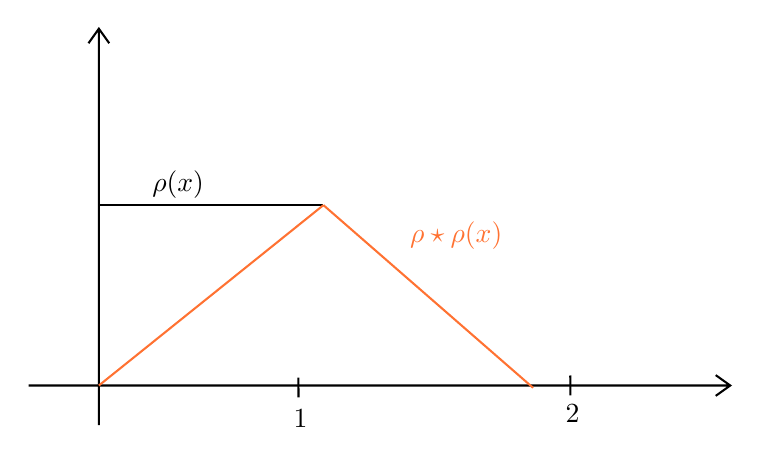
\begin{tikzpicture}[x=0.75pt,y=0.75pt,yscale=-1,xscale=1]
		%uncomment if require: \path (0,300); %set diagram left start at 0, and has height of 300
		
		%Shape: Axis 2D [id:dp8508806841135094] 
		\draw  (50,246.9) -- (388,246.9)(83.8,75) -- (83.8,266) (381,241.9) -- (388,246.9) -- (381,251.9) (78.8,82) -- (83.8,75) -- (88.8,82)  ;
		%Straight Lines [id:da16916887281741155] 
		\draw    (84,160) -- (192,160) ;
		
		
		%Straight Lines [id:da9049951895649381] 
		\draw [color={rgb, 255:red, 255; green, 114; blue, 50 }  ,draw opacity=1 ]   (83.8,246.9) -- (192,160) ;
		
		
		%Straight Lines [id:da21444674738376057] 
		\draw [color={rgb, 255:red, 255; green, 114; blue, 50 }  ,draw opacity=1 ]   (192,160) -- (293,248) ;
		
		
		%Straight Lines [id:da3378006631805073] 
		\draw    (179.92,243.08) -- (180,252.67) ;
		
		
		%Straight Lines [id:da715576960846674] 
		\draw    (310.92,242.08) -- (311,251.67) ;
		
		
		
		% Text Node
		\draw (122,150) node   {$\rho ( x)$};
		% Text Node
		\draw (256,174.67) node [color={rgb, 255:red, 255; green, 114; blue, 50 }  ,opacity=1 ]  {$\rho \star \rho ( x)$};
		% Text Node
		\draw (181,262.67) node   {$1$};
		% Text Node
		\draw (312,260.67) node   {$2$};
		
		
		\end{tikzpicture}
	\end{center}
	\begin{center}
		
		
		\tikzset{every picture/.style={line width=0.75pt}} %set default line width to 0.75pt        
		
		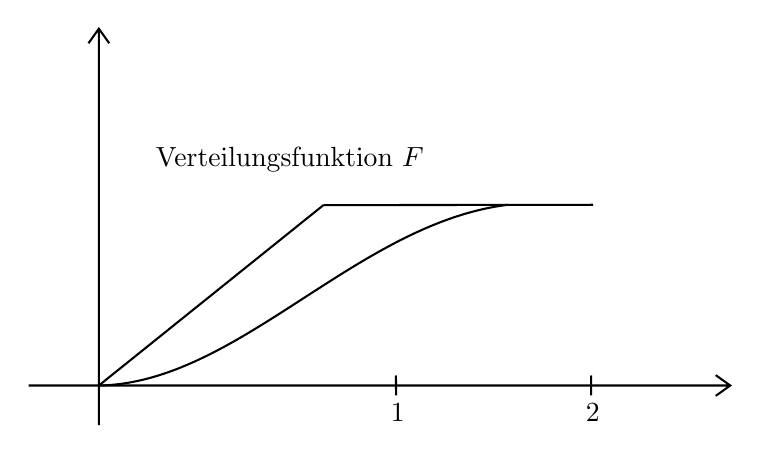
\begin{tikzpicture}[x=0.75pt,y=0.75pt,yscale=-1,xscale=1]
		%uncomment if require: \path (0,300); %set diagram left start at 0, and has height of 300
		
		%Shape: Axis 2D [id:dp9744249503209287] 
		\draw  (31,193.9) -- (369,193.9)(64.8,22) -- (64.8,213) (362,188.9) -- (369,193.9) -- (362,198.9) (59.8,29) -- (64.8,22) -- (69.8,29)  ;
		%Straight Lines [id:da04303841222166549] 
		\draw [fill={rgb, 255:red, 247; green, 9; blue, 9 }  ,fill opacity=1 ]   (64.8,193.9) -- (173,107) ;
		
		
		%Straight Lines [id:da9935141331554764] 
		\draw    (173,107) -- (302.92,106.83) ;
		
		
		%Curve Lines [id:da5574713559730453] 
		\draw    (64.8,193.9) .. controls (131.92,192.83) and (188.88,115.75) .. (261.92,106.83) ;
		
		
		%Straight Lines [id:da5561757729548006] 
		\draw    (207.92,189.08) -- (208,198.67) ;
		
		
		%Straight Lines [id:da41564219518446843] 
		\draw    (301.92,189.08) -- (302,198.67) ;
		
		
		
		% Text Node
		\draw (208.83,207.17) node   {$1$};
		% Text Node
		\draw (302.83,207.17) node   {$2$};
		% Text Node
		\draw (156.83,85.17) node  [align=left] {Verteilungsfunktion $\displaystyle F$};
		
		
		\end{tikzpicture}
	\end{center}
\end{example}
